\documentclass[11pt]{article}
\usepackage[utf8]{inputenc}
\usepackage[brazilian]{babel}
\usepackage{graphicx}
\usepackage[a4paper, top={.4in}, bottom={.65in}]{geometry}
\usepackage{subfig}
\usepackage{makecell}
\usepackage{textcomp}
\usepackage{gensymb}
\usepackage{tikz}
\usepackage{amsmath}
\usepackage{amssymb}

\begin{document}
\begin{center}
  \textbf{Experimento 06 -- PSI-3212} \\
  Natanael Magalhães Cardoso, nUSP: 8914122
\end{center}

\vspace{2cm}

\subsection*{Item 1.2}

\begin{figure}[h!]
  \centering
  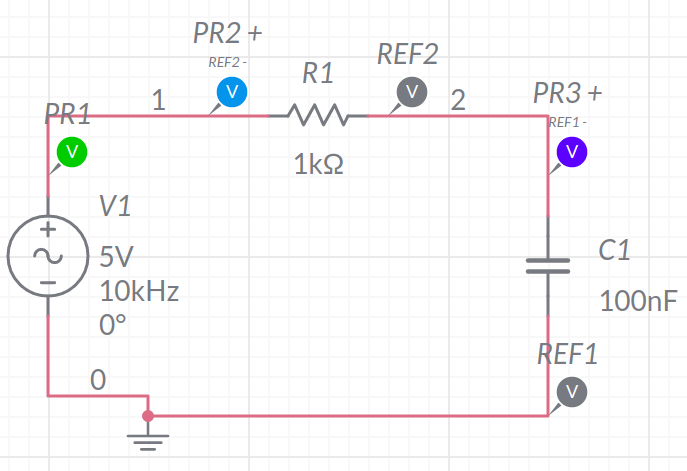
\includegraphics[width=.82\textwidth]{fig/1_circuito}
  \caption{Esquema do circuito}
  \label{fig:circ1}
\end{figure}

\subsection*{Item 1.2.a}

$$
  \left\|G(j\omega)\right\| = \left\|\frac{V_{S}}{V_{E}}\right\|
$$

onde $V_{S}$ é a tensão no capacitor e $V_{E}$ é a tensão no gerador.

$$
  \varphi(j\omega) = \varphi_{V_{S}} - \varphi_{V_{E}}
$$

onde $\varphi_{V_{S}}$ é a fase da tensão no capacitor e $\varphi_{V_{E}}$ é a fase da tensão no gerador.

\subsection*{Item 1.2.b}

$$
  \left\|G(j\omega)\right\| = \left\|\frac{4.22V}{5.0V}\right\| = 0.84
$$

\pagebreak

\subsection*{Itens 1.2.c, 1.2.d}

\begin{table}[h!]
  \centering
  \begin{tabular}{|c|c|c|c|c|}
    \hline
    $f$ [Hz] & $V_{E}$ [V] & $V_{S}$ [V] & $\varphi_{V_{S},V_{E}}$ [\textdegree] & $G(f)$ \\
    \hline
    10       & 3.54        & 3.53        & -0.36                                 & 0.997  \\
    50       & 3.54        & 3.53        & -1.81                                 & 0.997  \\
    100      & 3.54        & 3.52        & -3.61                                 & 0.99   \\
    300      & 3.54        & 3.45        & -10.70                                & 0.98   \\
    500      & 3.54        & 3.37        & -17.47                                & 0.95   \\
    700      & 3.54        & 3.22        & -23.91                                & 0.91   \\
    1k       & 3.54        & 2.98        & -32.31                                & 0.84   \\
    1.2k     & 3.54        & 2.81        & -37.14                                & 0.79   \\
    1.3k     & 3.54        & 2.73        & -39.41                                & 0.77   \\
    1.4k     & 3.54        & 2.65        & -41.47                                & 0.75   \\
    1.5k     & 3.54        & 2.57        & -43.40                                & 0.73   \\
    1.6k     & 3.54        & 2.48        & -45.19                                & 0.70   \\
    1.7k     & 3.54        & 2.40        & -46.98                                & 0.68   \\
    1.8k     & 3.54        & 2.33        & -48.50                                & 0.66   \\
    2k       & 3.54        & 2.19        & -51.51                                & 0.62   \\
    3k       & 3.54        & 1.65        & -62.06                                & 0.47   \\
    6k       & 3.54        & 0.91        & -75.09                                & 0.26   \\
    10k      & 3.54        & 0.55        & -80.96                                & 0.16   \\
    \hline
  \end{tabular}
  \caption{Tabela com os valores de tensão, defasagem e ganho para cada valor de frequência obtidos pela simulação.}
  \label{tab:1-2}
\end{table}

\subsection*{Item 1.2.e}

\begin{table}[h!]
  \centering
  \begin{tabular}{|c|c|c|c|c|}
    \hline
    $f$ [Hz] & $\varphi_{V_{S},V_{E}}$ [\textdegree] & $G(f)$ \\
    \hline
    10       & -0.36                                 & 1.0    \\
    50       & -1.80                                 & 1.0    \\
    100      & -3.60                                 & 1.0    \\
    300      & -10.67                                & 0.98   \\
    500      & -17.44                                & 0.95   \\
    700      & -23.74                                & 0.92   \\
    1k       & -32.14                                & 0.85   \\
    1.2k     & -37.02                                & 0.80   \\
    1.3k     & -39.24                                & 0.77   \\
    1.4k     & -41.34                                & 0.75   \\
    1.5k     & -43.30                                & 0.73   \\
    1.6k     & -45.15                                & 0.71   \\
    1.7k     & -46.89                                & 0.68   \\
    1.8k     & -48.52                                & 0.66   \\
    2k       & -51.49                                & 0.62   \\
    3k       & -62.05                                & 0.47   \\
    6k       & -75.14                                & 0.25   \\
    10k      & -80.96                                & 0.16   \\
    \hline
  \end{tabular}
  \caption{Tabela com os valores teóricos de defasagem e ganho para cada valor de frequência obtidos pela planílha disponibilizada como \emph{material complementar}.}
  \label{tab:1-2e}
\end{table}

\pagebreak

\subsection*{Item 1.2.f}

\begin{figure}[h!]
  \centering
  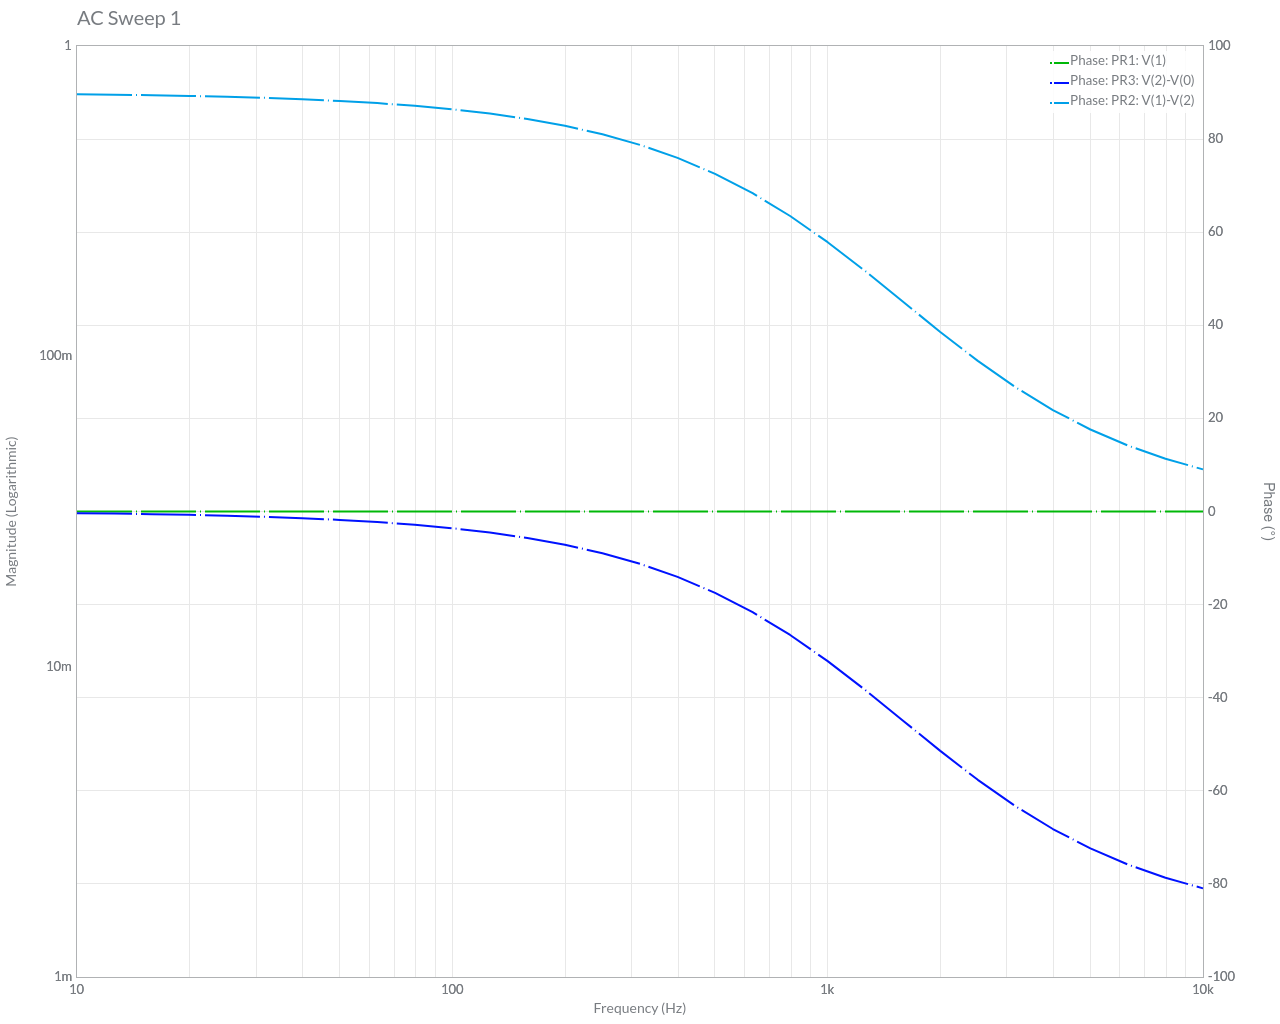
\includegraphics[width=.5\textwidth]{fig/1f_fase_sim}
  \caption{Gráfico da simulação do circuito (AC Sweep). Em verde, a defasagem $V_{E}$, em azul escuro a defasagem $V_{S}$. As curvas PR1, PR2 e PR3 são referentes às pontas de provas da figura \ref{fig:circ1}.}
\end{figure}

\subsubsection*{(i) Gráfico do Ganho}

\begin{figure}[h!]
  \centering
  \subfloat[]{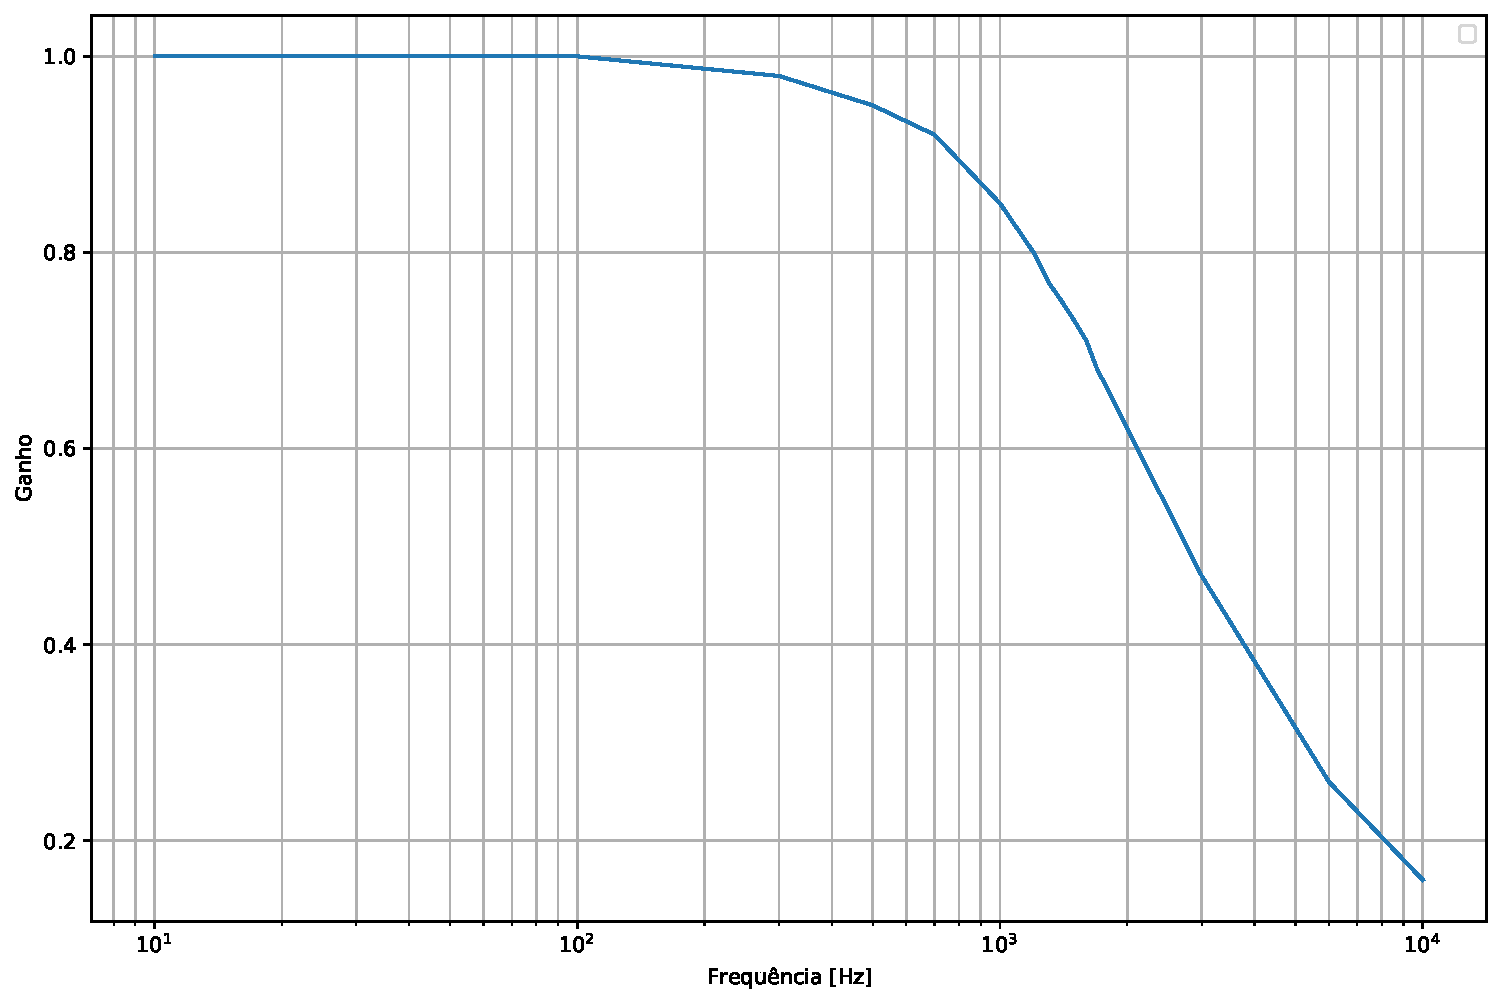
\includegraphics[width=.47\textwidth]{fig/1f_ganho_teo}}
  \qquad
  \subfloat[]{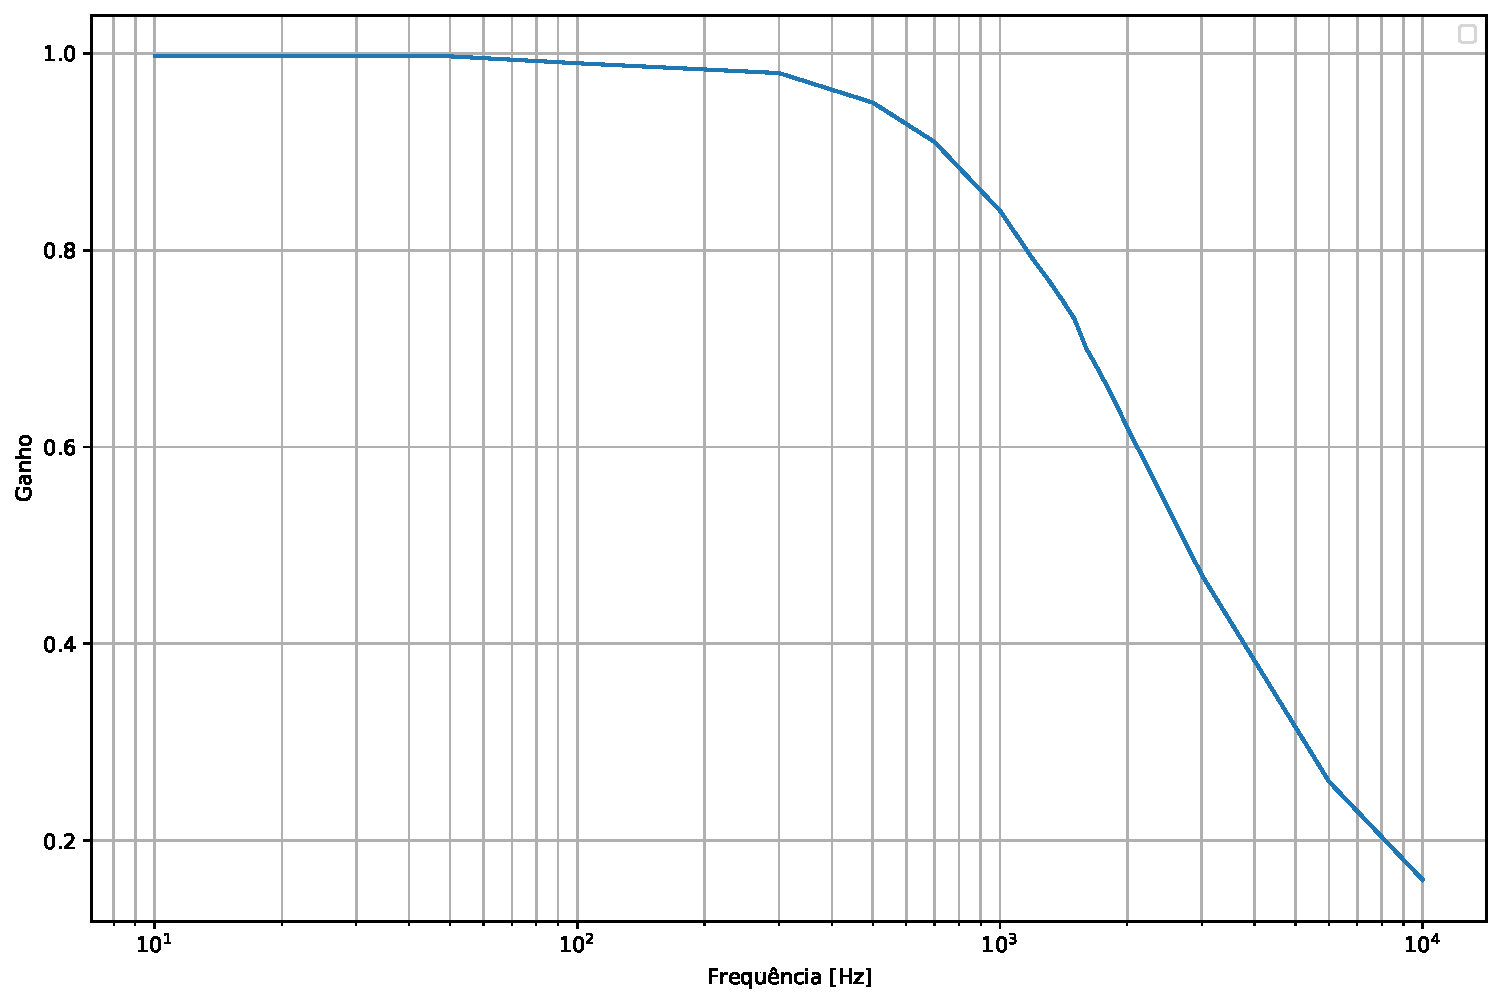
\includegraphics[width=.47\textwidth]{fig/1f_ganho}}
  \caption{A figura (a) mostra o gráfico teórico do ganho, plotado a partir da planilha disponibilizada como \emph{material complementar}. Já a figura (b) mostra o gráfico plotado a partir dos valores simulados da tabela \ref{tab:1-2}.}
\end{figure}

\subsubsection*{(ii) Gráfico da Fase}

\begin{figure}[h!]
  \centering
  \subfloat[]{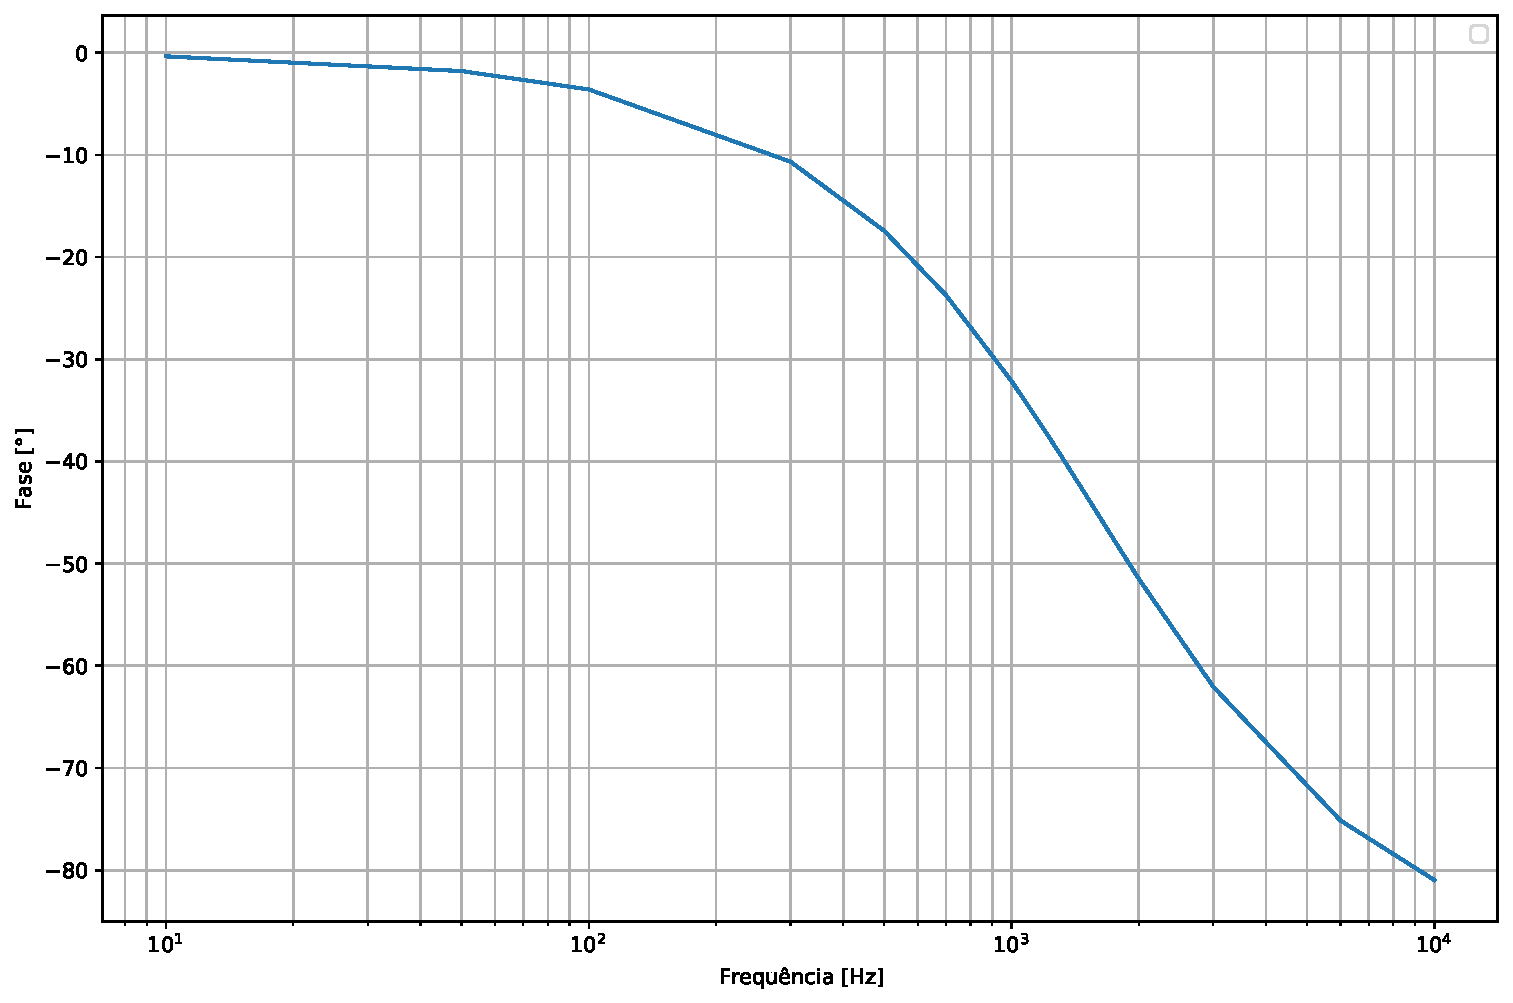
\includegraphics[width=.47\textwidth]{fig/1f_fase_teo}}
  \qquad
  \subfloat[]{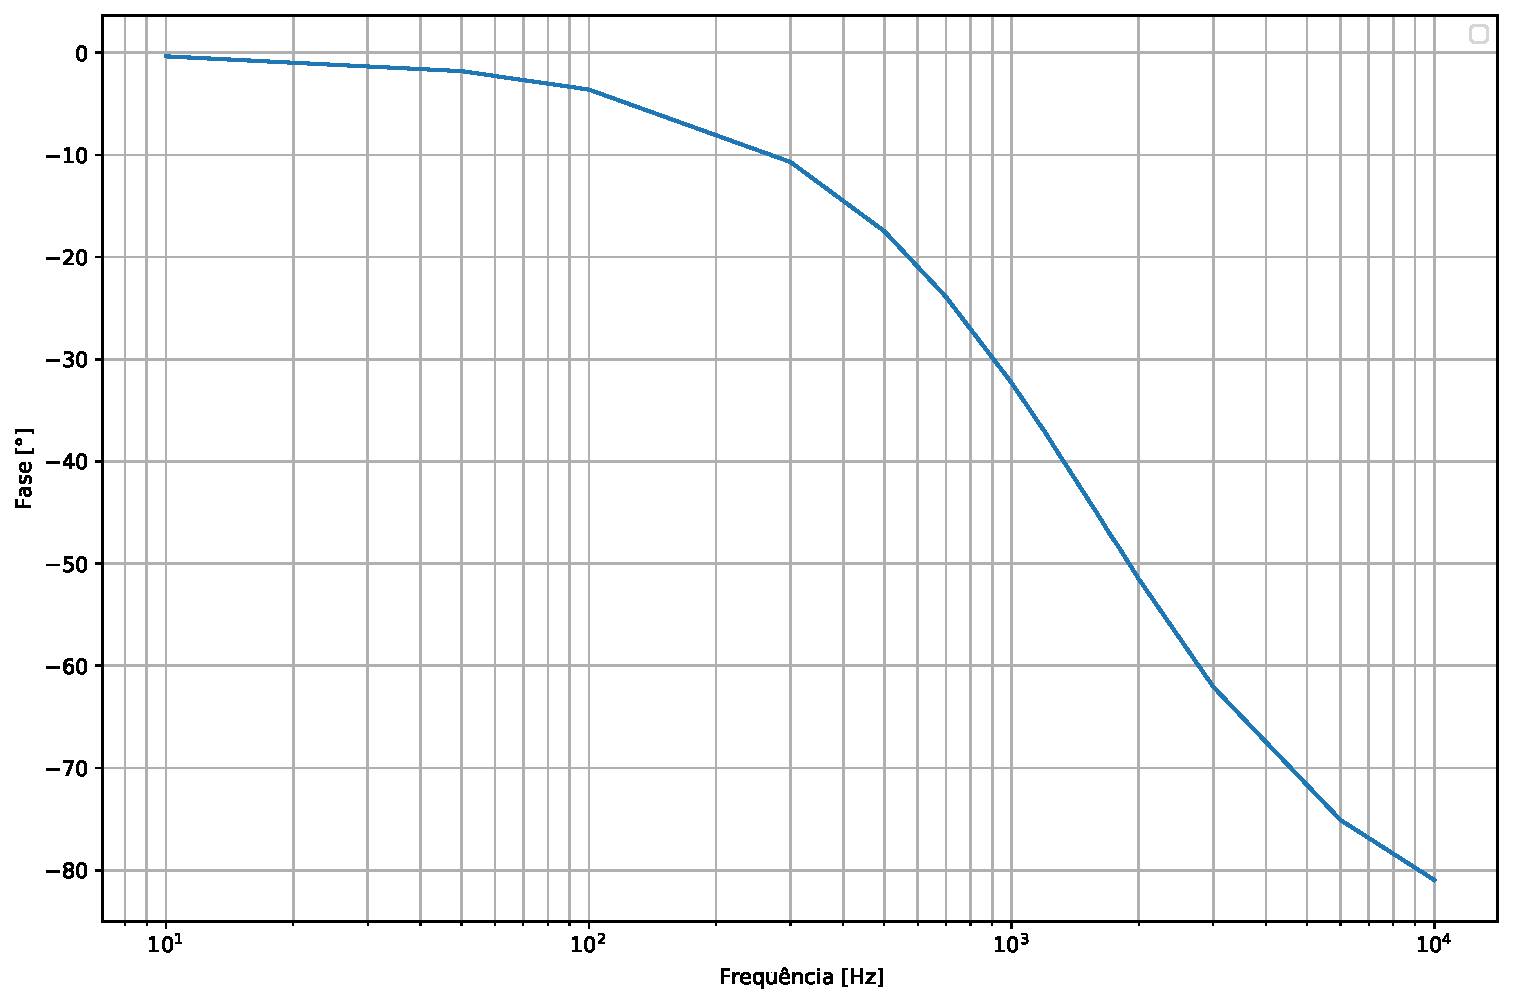
\includegraphics[width=.47\textwidth]{fig/1f_fase}}
  \caption{A figura (a) mostra o gráfico teórico da defasagem, plotado a partir da planilha disponibilizada como \emph{material complementar}. Já a figura (b) mostra o gráfico plotado a partir dos valores simulados da tabela \ref{tab:1-2}.}
\end{figure}

\subsection*{Item 1.2.g}

As curvas teóricas e simuladas são muito parecidas. O modelo é adequado.

\subsection*{Item 1.2.h}

Na tabela \ref{tab:1-2}, o ponto mais próximo de $45\degree$ na coluna de defasagem está na $12^{a}$ linha. Para esta fase, a frequência vale 1.6 kHz. Portanto,
$$
  f_{c} = 1.6\ k\textnormal{Hz}
$$

\subsection*{Item 1.2.i}

$$
  f_{c} = \frac{1}{2\pi RC} = \frac{1}{2\pi (1\ k\Omega)(100\ nF)} = 1591.55\ \textnormal{Hz}
$$

\subsection*{Item 1.2.j}

A determinação da frequência de corte pelo valor mais próximo da tabela \ref{tab:1-2} foi próximo ao valor calculado pela equação do item anterior.

$$
  \epsilon = \left\|\frac{1600 - 1591.55}{1591.55}\right\| \cdot 100 = 0.53\%
$$

\subsection*{Item 1.2.k}

Uma das aplicações deste circuito é usá-lo como um filtro.

\subsection*{Item 2}

Observação: O item 2 do \emph{Guia Experimental} não informa os valores de todos os componentes. Por isso, eu usei os valores descritos no item 2 da \emph{Introdução Teórica}.

\begin{figure}[h!]
  \centering
  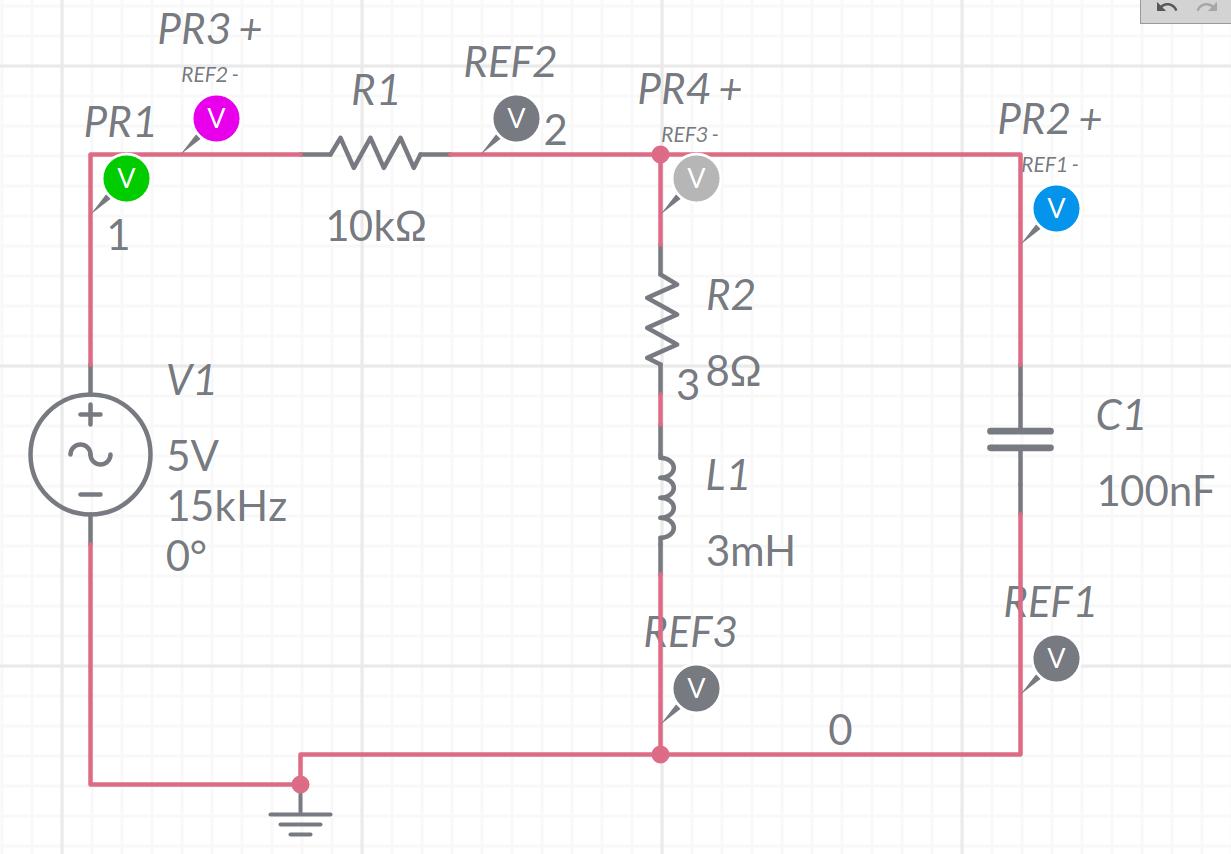
\includegraphics[width=.82\textwidth]{fig/2_circuito}
  \caption{Esquema do circuito com os medidores de tensão}
  \label{fig:circ2}
\end{figure}

\subsection*{Item 2.1.a}

Equações (11) e (12)

\pagebreak

\subsection*{Itens 2.1.b, 2.1.c}

\begin{figure}[h!]
  \centering
  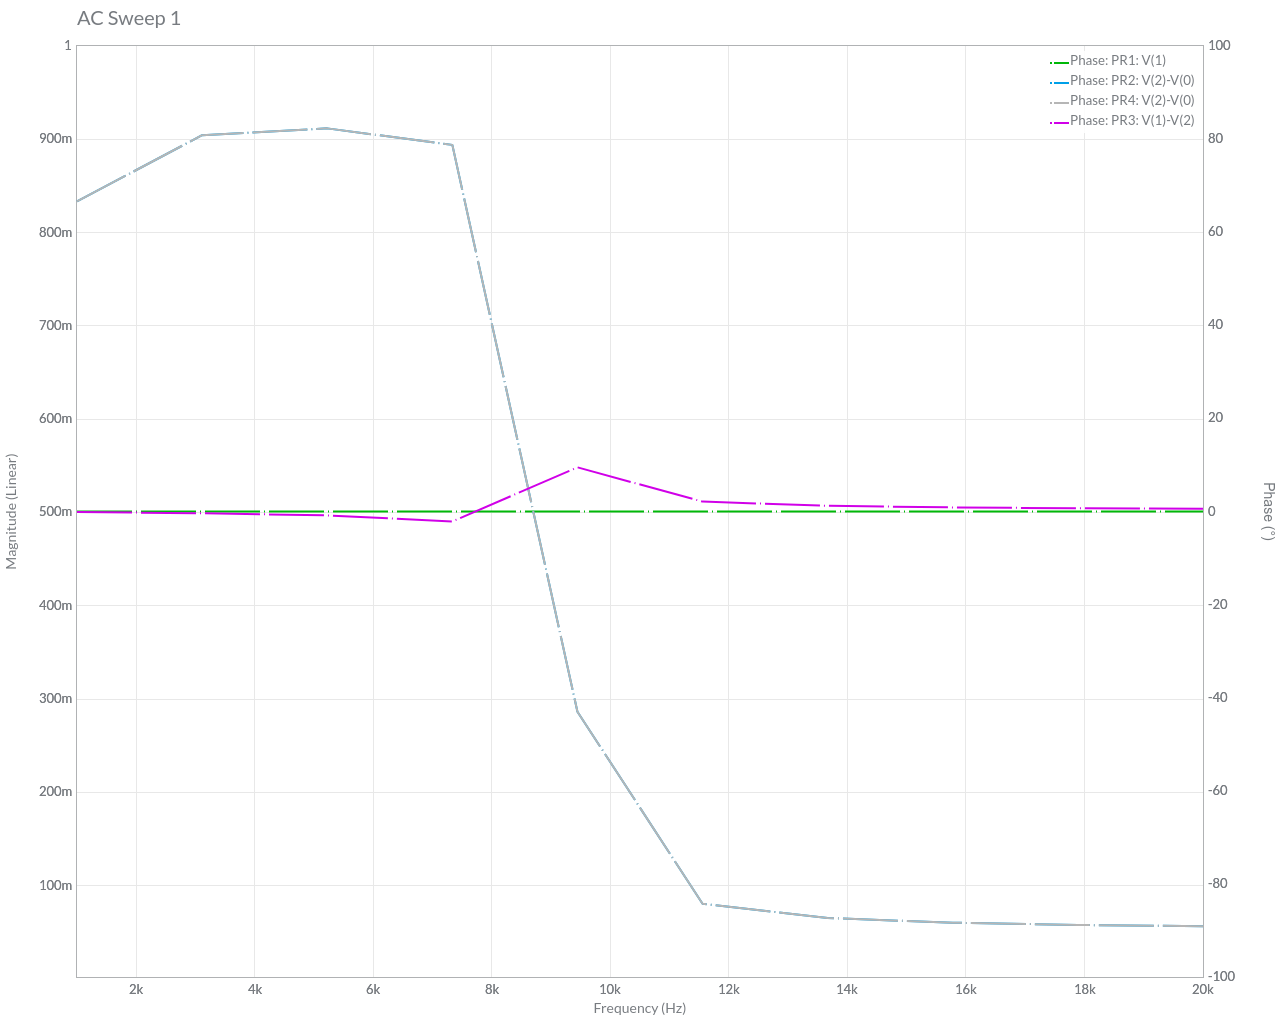
\includegraphics[width=.72\textwidth]{fig/2_sweep}
  \caption{Gráfico da fase gerado pela simulação AC Sweep. Os valoes PR\{1, 2, 3, 4\} da legenda são referentes aos medidores da figura \ref{fig:circ2}. PR2 $\equiv$ PR4.}
  \label{fig:2-sweep}
\end{figure}

\begin{table}[h!]
  \centering
  \begin{tabular}{|c|c|c|c|c|}
    \hline
    $f$ [Hz] & $V_{E}$ [${V_{RMS}}$] & $V_{S}$ [$V_{RMS}$]  & $\varphi_{V_{S},V_{E}}$ [\textdegree] & $\left\|G(f)\right\|$ \\
    \hline
    1k       & 3.54                  & $7.18 \cdot 10^{-3}$ & 66.60                                 & $2.03 \cdot 10^{-3}$  \\
    3k       & 3.54                  & $1.98 \cdot 10^{-2}$ & 80.09                                 & $5.59 \cdot 10^{-3}$  \\
    5k       & 3.54                  & $4.28 \cdot 10^{-2}$ & 82.16                                 & $1.21 \cdot 10^{-2}$  \\
    7k       & 3.54                  & $1.12 \cdot 10^{-1}$ & 79.33                                 & $3.16 \cdot 10^{-2}$  \\
    8k       & 3.54                  & $2.34 \cdot 10^{-1}$ & 39.82                                 & $6.61 \cdot 10^{-2}$  \\
    8.5k     & 3.54                  & $3.59 \cdot 10^{-1}$ & 11.39                                 & $1.01 \cdot 10^{-1}$  \\
    8.8k     & 3.54                  & $6.58 \cdot 10^{-1}$ & -6.29                                 & $1.86 \cdot 10^{-1}$  \\
    9k       & 3.54                  & $8.35 \cdot 10^{-1}$ & -17.81                                & $2.36 \cdot 10^{-1}$  \\
    9.2k     & 3.54                  & $9.55 \cdot 10^{-1}$ & -29.34                                & $2.70 \cdot 10^{-1}$  \\
    9.3k     & 3.54                  & $8.77 \cdot 10^{-1}$ & -34.72                                & $2.48 \cdot 10^{-1}$  \\
    9.4k     & 3.54                  & $7.47 \cdot 10^{-1}$ & -40.87                                & $2.11 \cdot 10^{-1}$  \\
    9.6k     & 3.54                  & $5.40 \cdot 10^{-1}$ & -46.19                                & $1.53 \cdot 10^{-1}$  \\
    10k      & 3.54                  & $3.23 \cdot 10^{-1}$ & -54.00                                & $9.12 \cdot 10^{-2}$  \\
    11k      & 3.54                  & $1.61 \cdot 10^{-1}$ & -73.54                                & $4.55 \cdot 10^{-2}$  \\
    12k      & 3.54                  & $1.09 \cdot 10^{-1}$ & -84.90                                & $3.08 \cdot 10^{-2}$  \\
    15k      & 3.54                  & $6.72 \cdot 10^{-2}$ & -87.96                                & $1.90 \cdot 10^{-2}$  \\
    20k      & 3.54                  & $4.17 \cdot 10^{-2}$ & -89.10                                & $1.18 \cdot 10^{-2}$  \\
    \hline
  \end{tabular}
  \caption{Tabela com os valores simulados para tensão de entrada, tensão de saída, fase e ganho.}
  \label{tab:2-1-c}
\end{table}

\pagebreak

\subsection*{Item 2.1.d}

\begin{table}[h!]
  \centering
  \begin{tabular}{|c|c|c|}
    \hline
    $f$ [Hz] & $\varphi_{V_{S},V_{E}}$ [\textdegree] & $\left\|G(f)\right\|$ \\
    \hline
    1k       & 66.60                                 & $2.07 \cdot 10^{-3}$  \\
    3k       & 80.62                                 & $6.39 \cdot 10^{-3}$  \\
    5k       & 82.34                                 & $1.34 \cdot 10^{-2}$  \\
    7k       & 79.97                                 & $3.12 \cdot 10^{-2}$  \\
    8k       & 74.13                                 & $6.06 \cdot 10^{-2}$  \\
    8.5k     & 65.10                                 & $1.02 \cdot 10^{-1}$  \\
    8.8k     & 51.21                                 & $1.61 \cdot 10^{-1}$  \\
    9k       & 30.99                                 & $2.27 \cdot 10^{-1}$  \\
    9.2k     & -4.12                                 & $2.73 \cdot 10^{-1}$  \\
    9.3k     & -22.73                                & $2.56 \cdot 10^{-1}$  \\
    9.4k     & -37.70                                & $2.23 \cdot 10^{-1}$  \\
    9.6k     & -56.34                                & $1.61 \cdot 10^{-1}$  \\
    10k      & -71.80                                & $9.62 \cdot 10^{-2}$  \\
    11k      & -82.23                                & $4.73 \cdot 10^{-2}$  \\
    12k      & -85.31                                & $3.19 \cdot 10^{-2}$  \\
    15k      & -88.06                                & $1.70 \cdot 10^{-2}$  \\
    20k      & -89.10                                & $1.01 \cdot 10^{-2}$  \\
    \hline
  \end{tabular}
  \caption{Valor térioricos da fase e do ganho para o circuito obtidos pela planilha.}
\end{table}


\subsection*{Item 2.1.e}
\subsubsection*{Gráfico do Ganho}

\begin{figure}[h!]
  \centering
  \subfloat[]{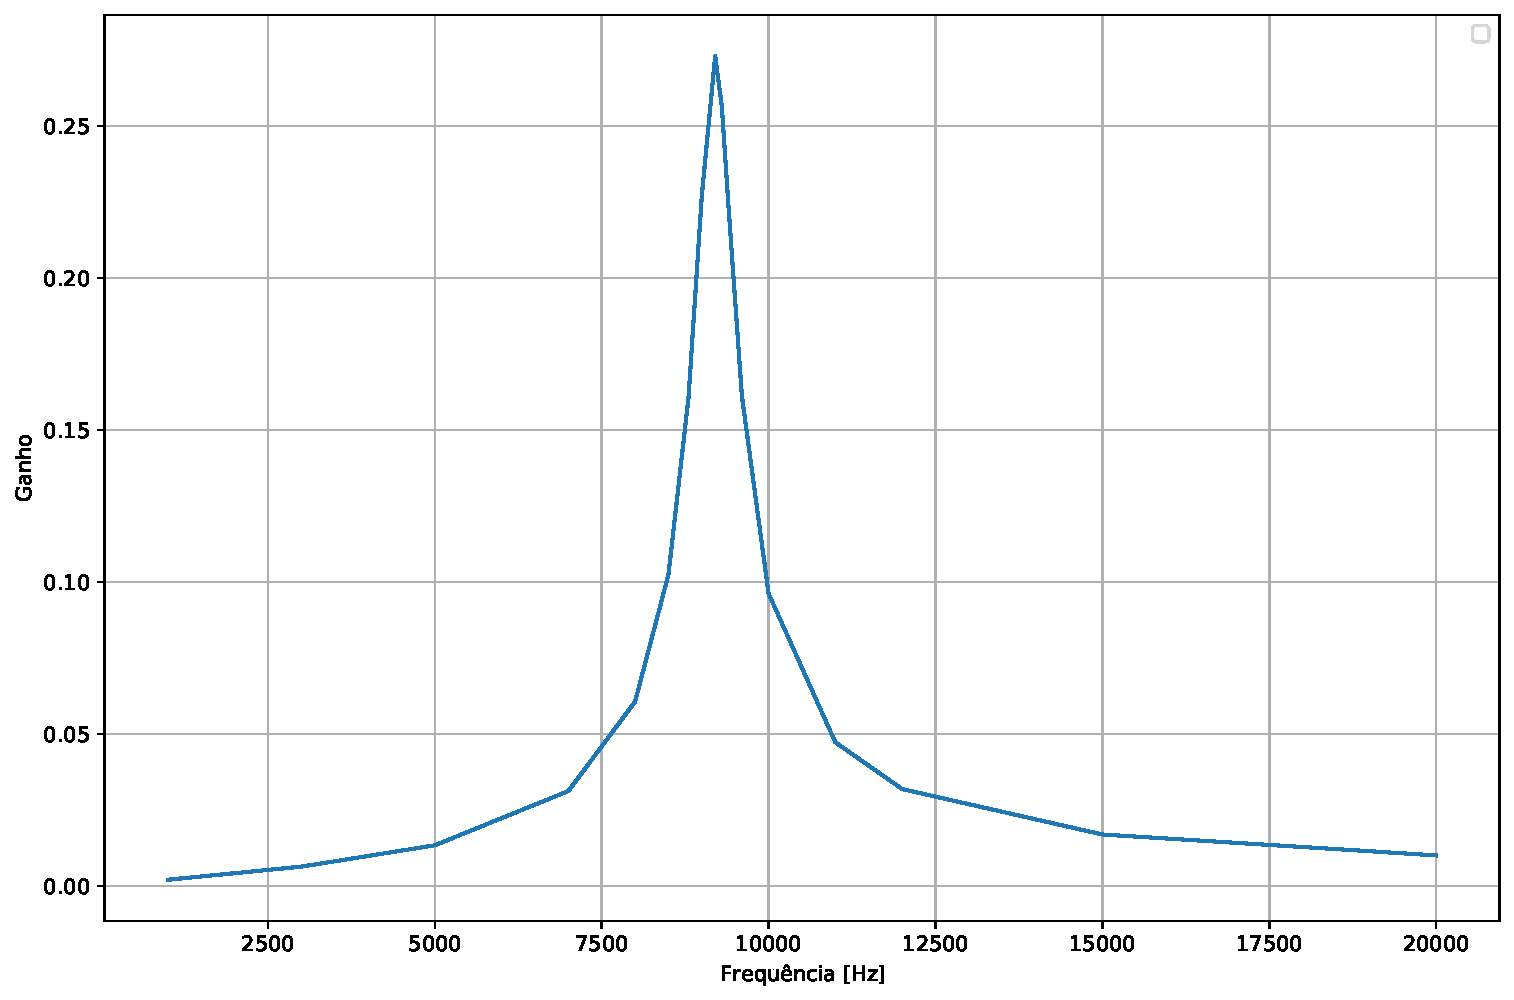
\includegraphics[width=.47\textwidth]{fig/2_ganho_teo}}
  \qquad
  \subfloat[]{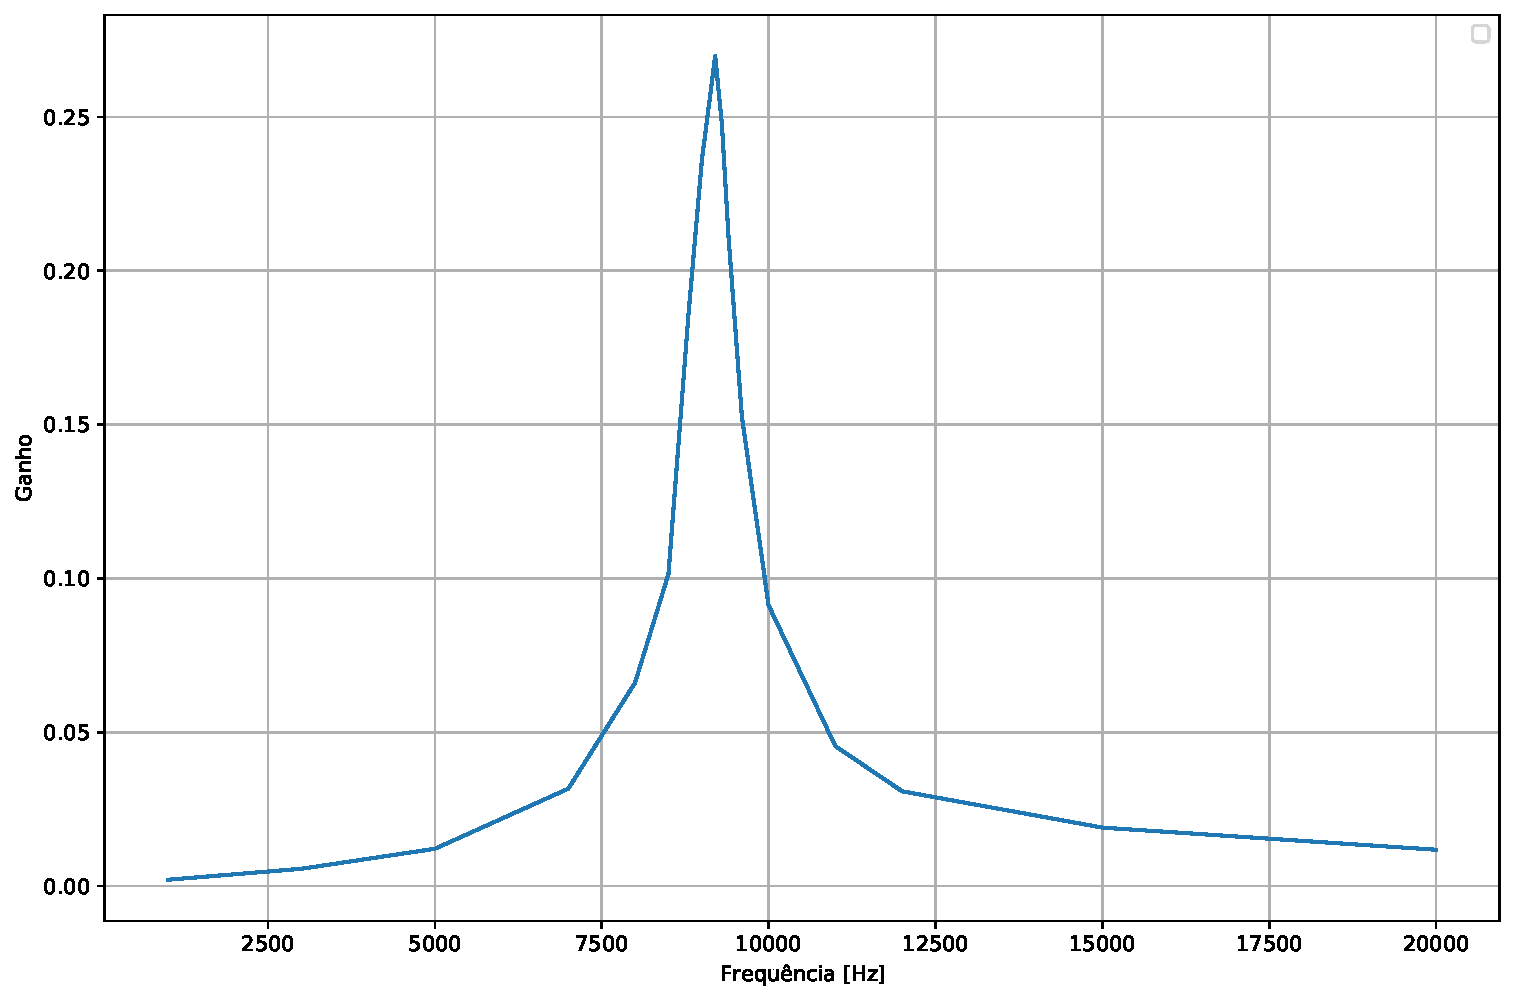
\includegraphics[width=.47\textwidth]{fig/2_ganho_exp}}
  \caption{A figura (a) mostra o gráfico teórico do ganho, plotado a partir da planilha disponibilizada como \emph{material complementar}. Já a figura (b) mostra o gráfico plotado a partir dos valores simulados da tabela \ref{tab:2-1-c}.}
\end{figure}

\pagebreak

\subsubsection*{Gráfico da Fase}

\begin{figure}[h!]
  \centering
  \subfloat[]{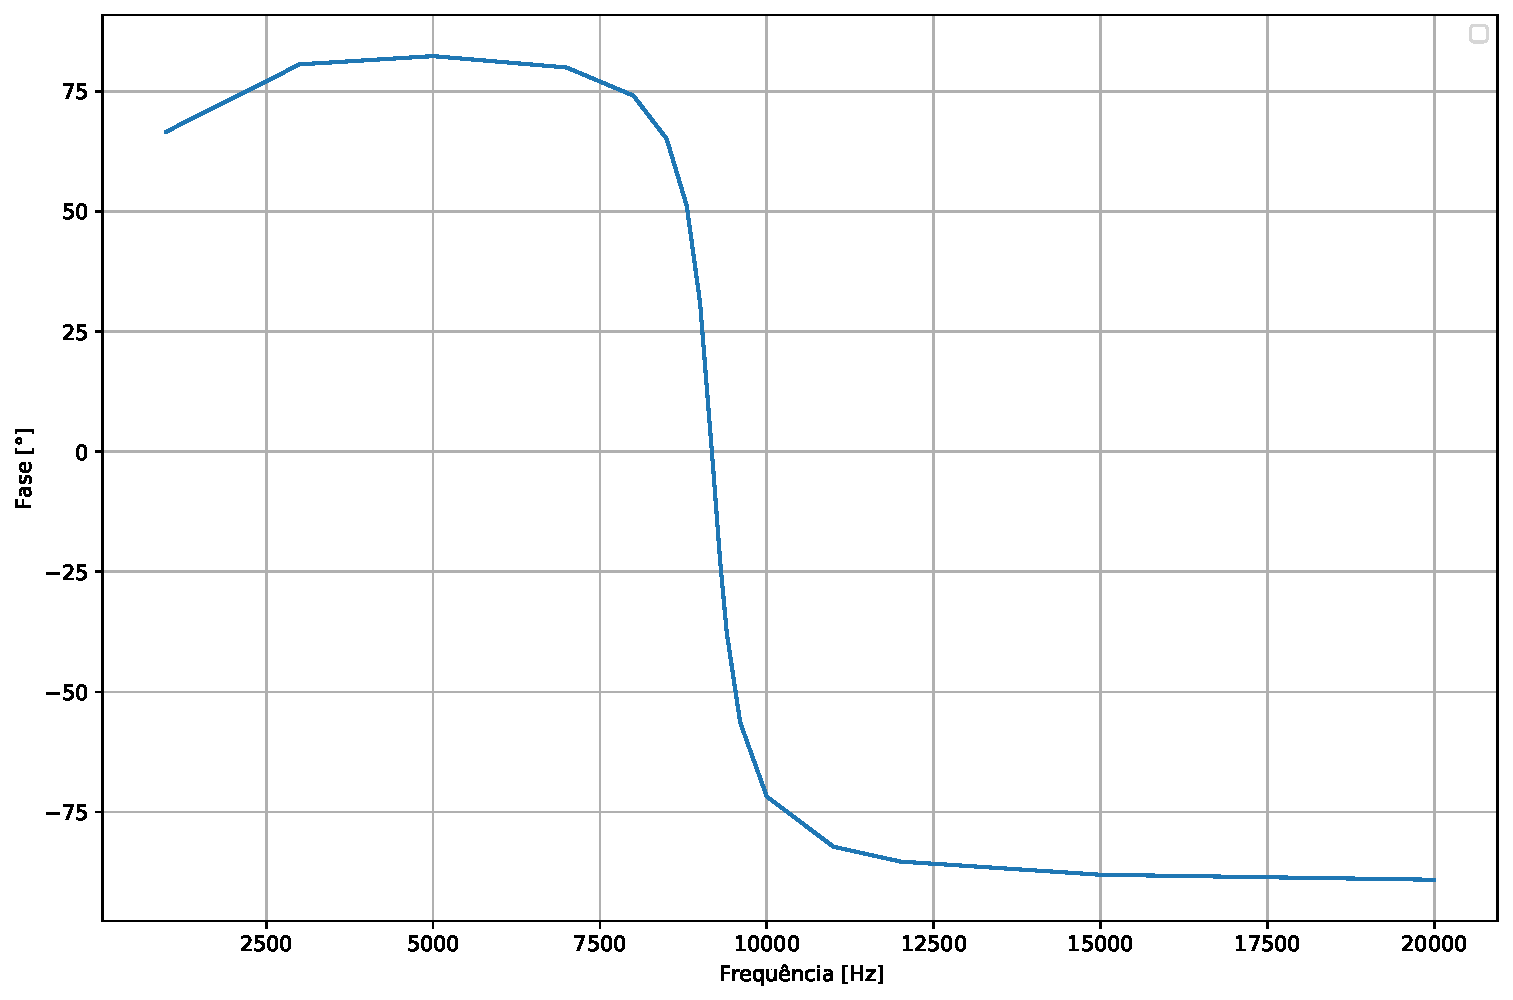
\includegraphics[width=.47\textwidth]{fig/2_fase_teo}}
  \qquad
  \subfloat[]{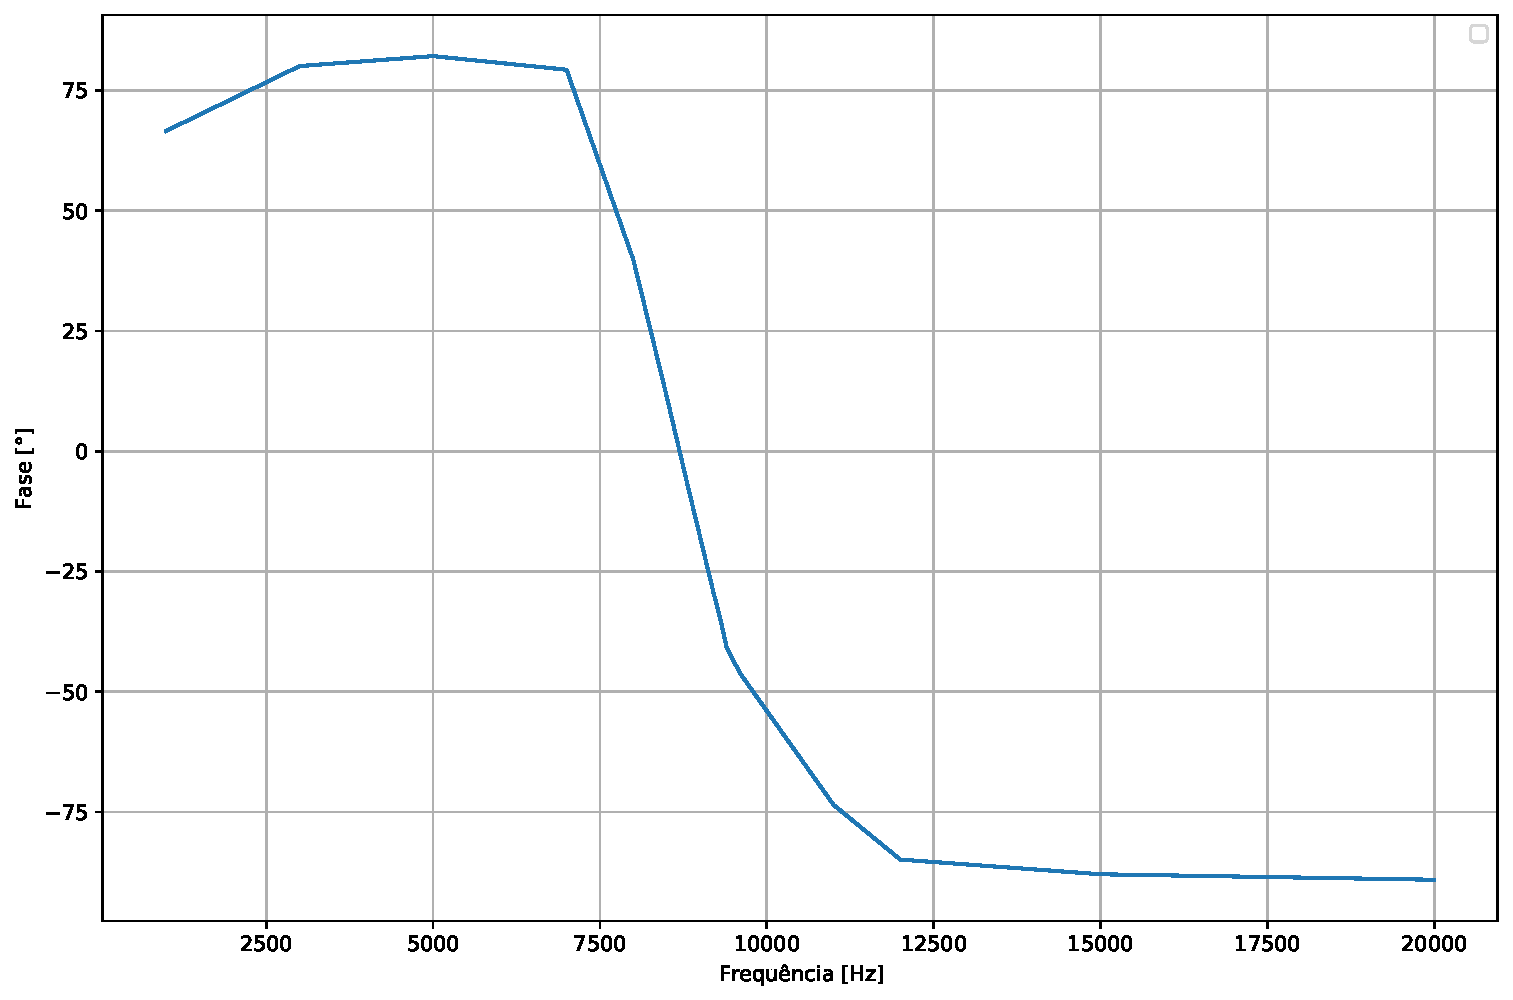
\includegraphics[width=.47\textwidth]{fig/2_fase_exp}}
  \caption{A figura (a) mostra o gráfico teórico da fase, plotado a partir da planilha disponibilizada como \emph{material complementar}. Já a figura (b) mostra o gráfico plotado a partir dos valores simulados da tabela \ref{tab:2-1-c}.}
\end{figure}

\subsection*{Item 2.1.f}

\begin{figure}[h!]
  \centering
  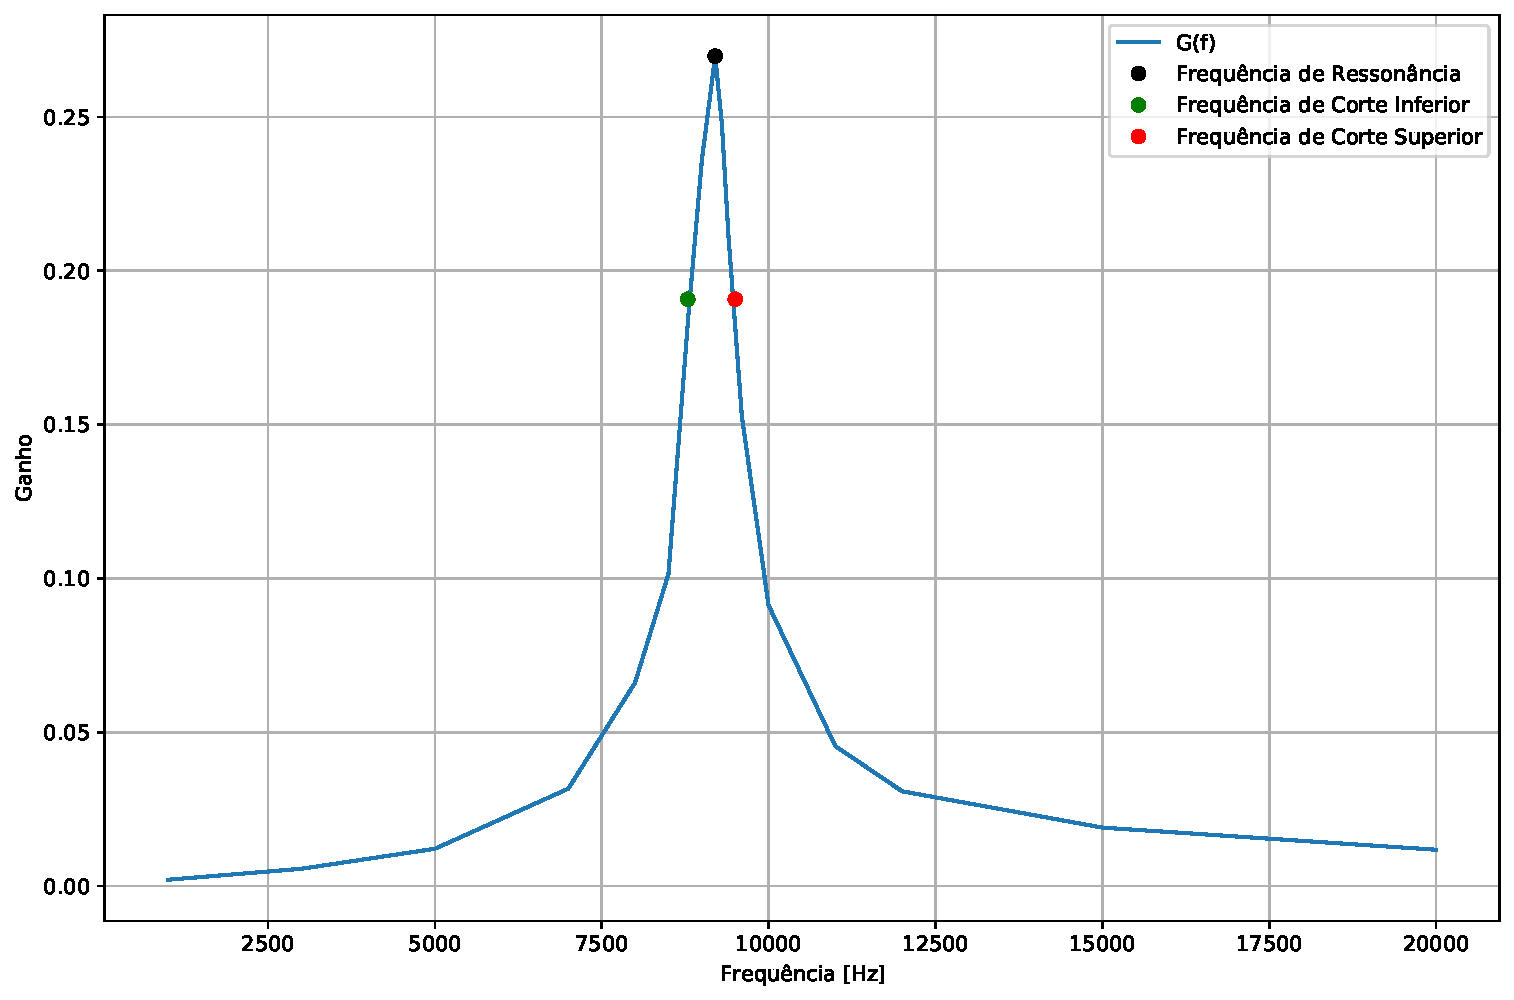
\includegraphics[width=.82\textwidth]{fig/2-1f}
  \caption{Gráfico de $G(f)$ indicando os pontos de intersecção da frequência de ressonância e de corte com a curva $G(f)$.}
\end{figure}

Para obter o valor da frequência de ressonância a partir dos dados experimentais, basta olhar para o valor máximo de $G_{f}$ e ver a frequência naquele ponto.

$$
  G_{R} = G(f_{R}) = \max(G) \approx 0.27 \Rightarrow f_{R} \approx 9.2\ \textnormal{kHz}
$$

Com o valor do ganho mámixo, é possível obter as frequências de corte olhando para os valores de frequência no conjunto $\{f_{C} \in \mathbb{R} : G(f_{C}) = G_{R}/\sqrt{2}\}$.

$$
  G_{C} = \frac{G_{R}}{\sqrt{2}} \approx 0.19 \Rightarrow
  \begin{cases}
    f_{C_{1}} \approx 8.8\ \textnormal{kHz} \\
    f_{C_{2}} \approx 9.5\ \textnormal{kHz}
  \end{cases}
$$

A faixa de passagem é dada por

$$
  \Delta f = f_{C_{2}} - f_{C_{1}} = (9.5 - 8.8)\ \textnormal{kHz} = 0.7\ \textnormal{kHz}
$$

O índice de mérito é dado por

$$
  Q = \frac{f_{R}}{f_{C_{2}} - f_{C_{1}}} = \frac{9.2\ \textnormal{kHz}}{(9.5\ \textnormal{kHz}) - (8.8\ \textnormal{kHz})} \approx 13.14
$$

\subsection*{Item 2.1.g}

Calculando a frequência de ressonância

$$
  f_{R} = \frac{1}{2\pi \sqrt{LC}} = \frac{1}{2\pi \sqrt{(3\ \textnormal{mH})(100\ \textnormal{nF})}} = 9.19\ \textnormal{kHz}
$$

O erro é dado por

$$
  \epsilon = \left\|\frac{9200 - 9189}{9189}\right\| \cdot 100 = 0.12\%
$$

\subsection*{Item 2.1.h}

A desafasem é estritamente decrescente no intervalo da faixa de passagem. Neste intervalo, o módulo da fase vai de 0\textdegree\ a 45\textdegree . Depois da frequência de corte superior, o módulo da fase aumenta com uma taxa menor.

\subsection*{Item 2.1.i}

A fase tenderia a 90\textdegree.

\end{document}
